\documentclass[a4paper]{article}

%% Language and font encodings
\usepackage[english]{babel}
\usepackage[utf8x]{inputenc}
\usepackage[T1]{fontenc}

%% Sets page size and margins
\usepackage[a4paper,top=3cm,bottom=2cm,left=3cm,right=3cm,marginparwidth=1.75cm]{geometry}

%% Useful packages
\usepackage{amsmath}
\usepackage{graphicx}
\usepackage[colorinlistoftodos]{todonotes}
\usepackage[colorlinks=true, allcolors=blue]{hyperref}
\usepackage{float}

\title{Cryogenic Buffer Gas Beam}
\author{Gary Chen}

\begin{document}
\maketitle

\section{Introduction to Buffer Gas Beams}

To reach reaction temperatures in the regime of 10K from a beam of molecules with trapped ions, a cryogenic buffer gas beam (CBGB) of neon with entrained water is employed. Numerous methods of creating cold beams of molecules exist, from Zeeman decelerators \cite{Narevicius2008}, Stark decelerators, to cryogenic buffer gas beams (CBGB). CBGB's in particular have the benefit of being species agnostic, where the resultant beam properties are not dependent on the target species at hand, rather, the buffer gas species. \todo{Add citations for decelerators}

By holding a cell filled with a buffer gas of neon of helium above its vapor pressure, a volume of gas can be held at cryogenic temperatures. Other species of molecules are atoms may be introduced into the buffer gas cell via ablation, fill line, etc. The target species particles are then sympathetically cooled via collisions with the cold buffer gas. An aperture at one end of the cell allows for the extraction of the buffer gas and entrained target species into a beam. Regulating the buffer gas cell temperature to above 17K for neon, and 4K for helium, in high vacuum allows us to accumulate an appreciable stagnation number density.
\todo{Add graphic to show what a buffer gas beam is}

The Reynolds number is typically used to characterize the flow regime of the buffer gas beam. At the aperture of the buffer gas cell, the Reynolds number can be written as:

\begin{align} \label{e: reynolds}
Re & \approx \frac{2 d_{aperture}}{\lambda} \\
& \approx \frac{8\sqrt[]{2} \dot{N} \sigma}{d_{aperture} \bar{v}}
\end{align}

Where $d_{aperture}$ is the diameter of the aperture and $\lambda$ is the mean free path of the buffer gas particles \cite{Hutzler2012}.

\subsection{Beam Velocity}

At thermal equilibrium, the velocities inside the buffer gas cell follows a Maxwell Boltzmann distribution:

\begin{align} \label{e: mb_distribution}
f(v) & = \left(\frac{m}{2 \pi k T}\right)^{3/2}4 \pi v^2 e^{-\frac{m v^2}{2 k T}}
\end{align}

Where the mean velocity is:

\begin{align} \label{e: mb_mean}
\bar{v} & = \sqrt{\frac{8 k_B T}{\pi m}}
\end{align}

We may rewrite the distribution as a function of the mean velocity $\bar{v}$ into a simpler form .

\begin{align} \label{e: mb_simplified}
f(v) & = \frac{32}{\pi^2} \frac{v^2}{\bar{v}^3} e^{-4v^2/\pi \bar{v}^2}
\end{align}

To get the velocity distribution in the beam, we can calculate the distribution of particles incident on an aperture in the cell.

\begin{align}
f_{beam}(v) & = \frac{v}{\bar{v}}f(v)  \\
& = \frac{32}{\pi^2} \frac{v^3}{\bar{v}^4} e^{-4v^2/\pi \bar{v}^2}
\end{align}

For low Reynold's numbers (Re<1) the flow at the aperture is purely molecular, which means that there are few to no collisions. This allows us to continue to use the Maxwell-Boltzmann distribution to describe the forward velocity \cite{Hutzler2011c}.

\begin{align}
\bar{v}_\parallel & = \int_0^\infty v f(v) dv \approx 1.2 \bar{v}
\end{align}

The spread of the forward velocity of an effusive beam is the full width half max (FWHM) of the Maxwell-Boltzmann distribution: $\Delta\bar{v} \approx 1.5 \bar{v}$.

As one increases the Reynolds number, one can reach the supersonic regime (Re>100) where the velocity reaches $1.4\bar{v}$ \cite{Hutzler2011c}.

But as the flow regime nears the supersonic regime, forward collisions around the aperture cause boosting of the average velocity as well as a decrease in the velocity spread. Changing the flow regime may also change the ratio of species in the beam as well.

A helium buffer gas held at 4K will be slower than a neon gas held at 17K. Despite this, it is preferable to use neon as a buffer gas due to its ideal cryopumping properties. Helium requires large amounts of activated charcoal, also held at low temperatures, to effectively cryopump. These volumes of charcoal can then become saturated and require purging, limiting one's operating time. Neon on the other hand, only requires a metal surface lower than 17K to create neon ice. The neon ice surface will then act as a cryopump for more neon gas as well, allowing for hours of continuous operation with no appreciable build up of background gas. Our experiment uses neon as a buffer gas for its technical simplicity, the lower achievable temperature with the helium does not yield dramatic gains in the final reaction temperature.

\subsection{Density and Extraction}

The stagnation density inside the buffer gas cell is a function of the physical dimensions of the cell and the number flow rate into the cell. High stagnation densities allows for high densities of reactants at the ion trap center, but can push the beam into an unwanted flow regime where the beam properties are not what one wants. Experimentally, it's preferable to use volumetric flow rates when operating the apparatus, but for calculations, that needs to translate to number flow rate using the ideal gas law:

\begin{align}
\dot{N} = \frac{P f}{k_B T}
\end{align}

where $P$ is pressure and $f$ is the volumetric flow rate, this translates to about $4\times10^{17} \text{ particles} \cdot \text{s}^{-1}$ for 1 SCCM of gas flow. By solving for the number density in the flow out of an aperture with molecular flow, we find that the stagnation density within the cell can be shown as:

\begin{align}
n_{b}=\frac{4 \dot{N}}{A_{aperture} \bar{v}}
\end{align}

In general, buffer gas beams operate with stagnation densities around $10^{15}-10^{17} cm^{-3}$. Outside of the cell, we can describe the density of the beam as a function of distance. \cite{Pauly}

\begin{align}
n(z)=\frac{n_o}{2}\left(1-\frac{z}{\sqrt{z^2+a^2}}\right)
\end{align}

Where $z$ is the distance from the aperture into the vacuum side, $n_o$ is the initial number density, $a$ is the radius of the aperture. In the far field, this goes to

\begin{align}
n(z)=\frac{n_o a^2}{4 z^2}
\end{align}

But there is something that we must consider, that is that we aren't seeing the full aperture while we are at all locations, we are actually seeing an appended area due to the inclusion of apertures and skimmers in the way. So in the calculation for $n(z)$, only $n_o$ has a dependence on the aperture size of the cell, $n(z)$ itself will have a set value defined by the smallest aperture in the beam path.

Sympathetic cooling occurs through collisions between the hot target species being introduced and the cryogenic buffer gas particles. The thermalization of the target species with the buffer gas particles is derived via momentum conservation of hard sphere collisions, where $\approx 10$ and $\approx 100$ collisions are needed to relax translational and rotational states to within a factor of 2 of the buffer gas temperature. Vibrational degrees of freedom may take upwards of $10^4$ collisions to fully thermalize is the elastic collision energy is much lower than the internal vibrational level. By finding the mean free path, we can consider the characteristic length the particles travel to be thermalized with the buffer gas, this is then compared to the characteristic length of the cell to determine the effectiveness of the cooling.

\begin{align}
\lambda = \frac{A_{aperture} \bar{v}}{4 f \sigma \sqrt{m_s/m_b}}
\end{align}

If a species is introduced into the buffer gas cell that has a lower vapor pressure than that is allowed at the current temperature, it will be lost when it comes in contact with the cell walls. The rate of this loss can be described as the  characteristic time of diffusion of a particle in the buffer gas to the physical dimensions of the cell set the diffusion time constant:

\begin{align}
\tau_{diff} = \frac{16}{9 \pi} \frac{A_{cell} n_{0,b} \sigma}{\bar{v}}
\end{align}

where $\sigma$ represents the collisional cross section for the buffer gas with the target species. On the other hand, we have the characteristic pump out time given by the conductance of a cell aperture:

\begin{align}
\tau_{pump}=\frac{4V_{cell}}{\bar{v}A_{aperture}}
\end{align}

By combining the $\tau_{diff}$ with the $\tau_{pump}$, we can get a dimensionless ratio, $\gamma$ that characterizes the extraction fraction out of the cell.

\begin{align}
\gamma = \frac{\tau_{diff}}{\tau_{pump}} = \frac{\sigma f}{L_{cell} \bar{v}} \label{e: gamma}
\end{align}

Notice that the $\gamma$ factor does not depend on aperture size, this is generally true, but increasing the aperture size will lower your number density within the cell, which then influences the characteristic length scale of thermalization. Larger apertures thus run the risk of not allowing your particles to fully thermalize in rotational/vibrational states. But decreasing the aperture size can make alignment as well as controlling the number density more difficult, as finer control over the flow rate is necessary for equivalent flow regimes.

\section{Experimental Apparatus}

The CBGB apparatus was homebuilt out of aluminum for the outer chamber as well as the inner 40K radiation shield. A Cryomech PT415 Pulse Tube Refrigerator with a remote head option was inserted into the chamber. A large bellows attachment connected the pulse tube cooler head to the chamber itself to isolate the chamber from the mechanical vibrations caused by the pulse tube cooler itself.

The pulse tube cooler itself has 2 cooling stages and a room temperature stage. The room temperature stage at the top is where 

\begin{figure}[H]
\centering
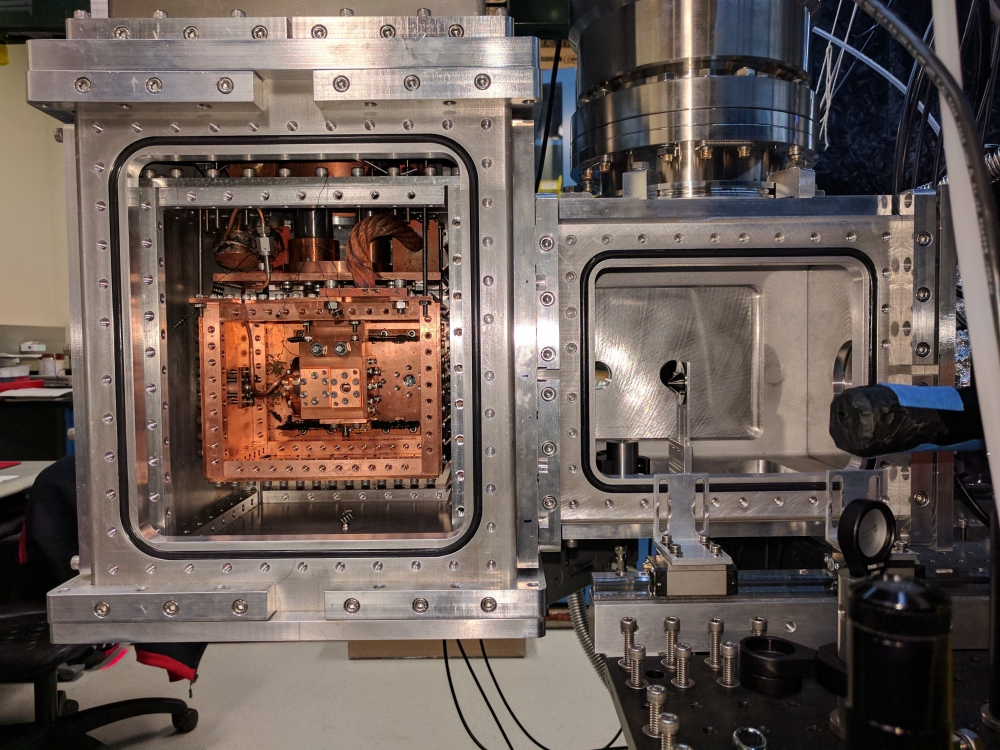
\includegraphics[width=1\textwidth]{beam_cross_section.jpg}
\caption{Cross sectional view of CBGB with side walls removed from the outer vacuum chamber, 40K aluminum radiation shield, and inner 4K cryopumping shield.}
\label{f: chamber}
\end{figure}

\begin{figure}[H]
\centering
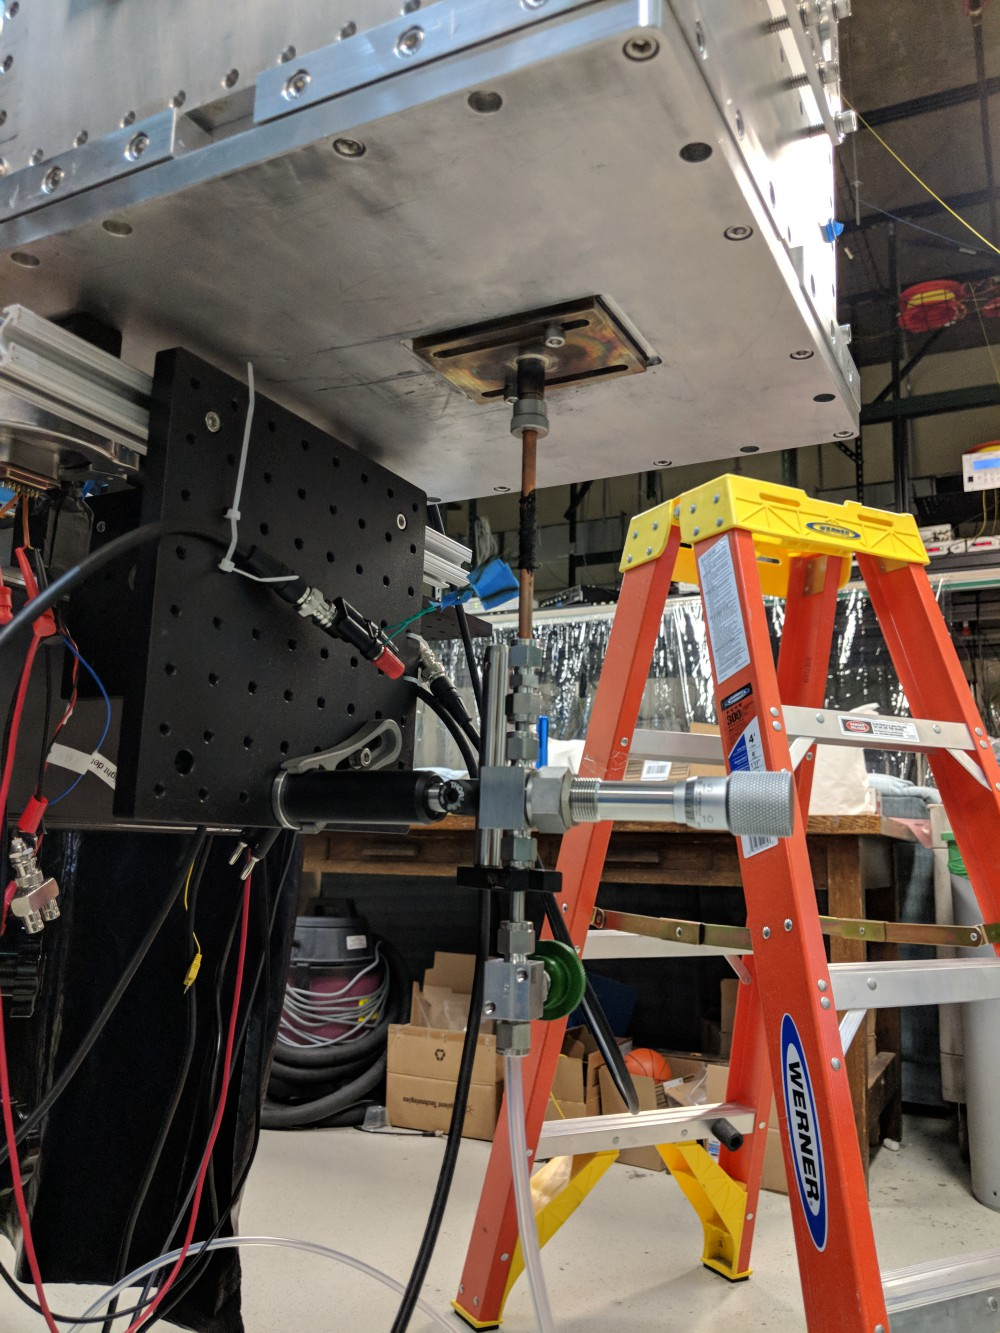
\includegraphics[width=.7\textwidth]{water_fill_outside.jpg}
\caption{The water fill line, sealed by an ultratorr fitting and heated by nichrome wire. A shut off valve and vernier valve are used to regulate the flow of water into the buffer gas cell.}
\label{f: outside}
\end{figure}

\begin{figure}[H]
\centering
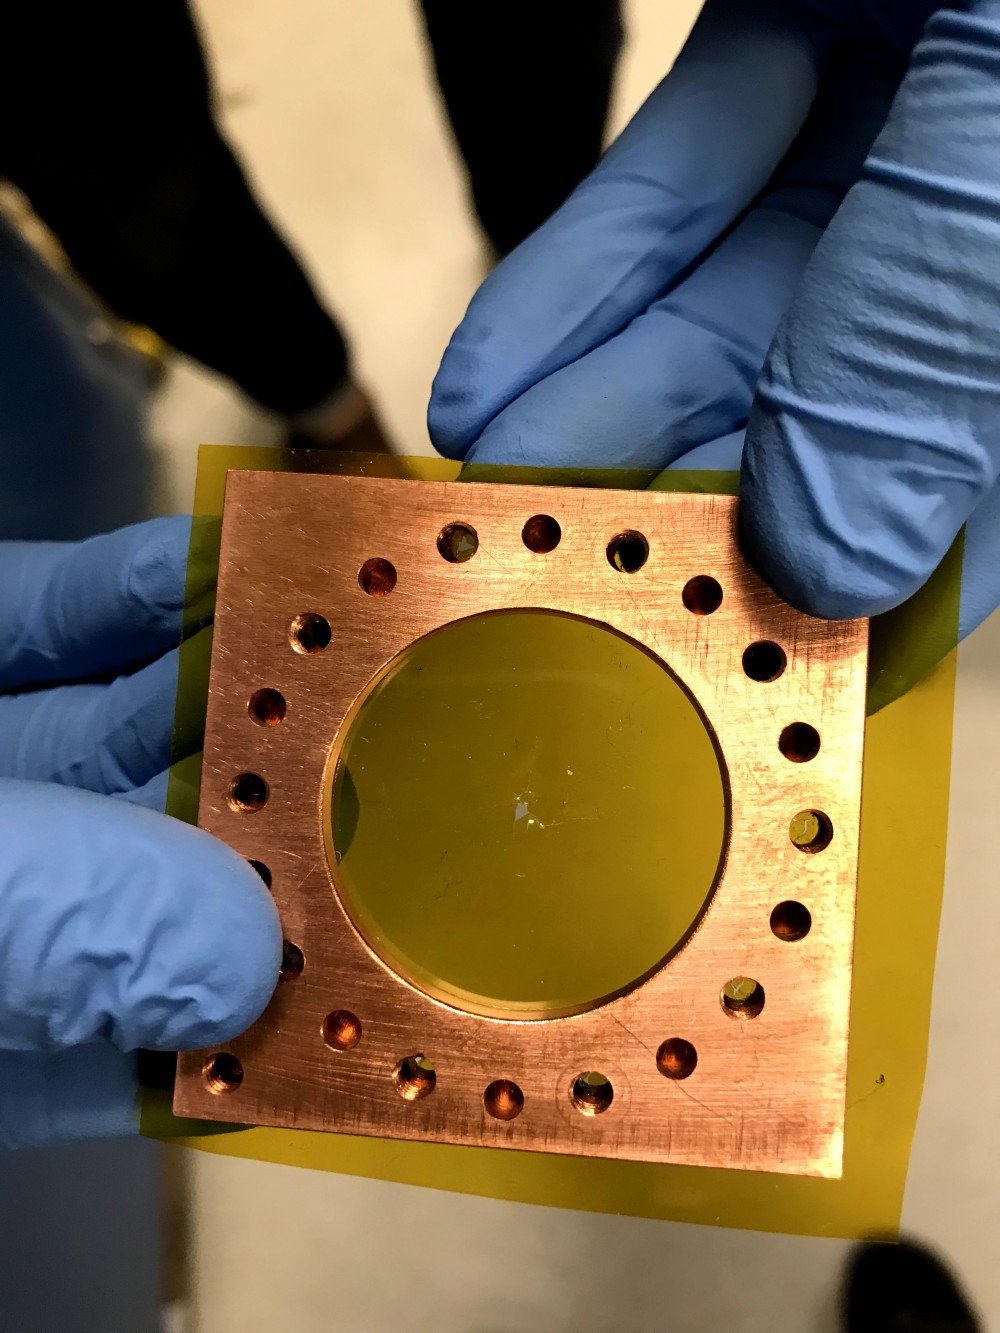
\includegraphics[width=.7\textwidth]{kapton.jpg}
\caption{A kapton film serves as the back wall of the buffer gas cell with a hole for the insertion of the water fill line. The kapton surface resists ice formation and allows for continuous operation with water for over 10 hours.}
\label{f: kapton}
\end{figure}

\begin{figure} [H]
\centering
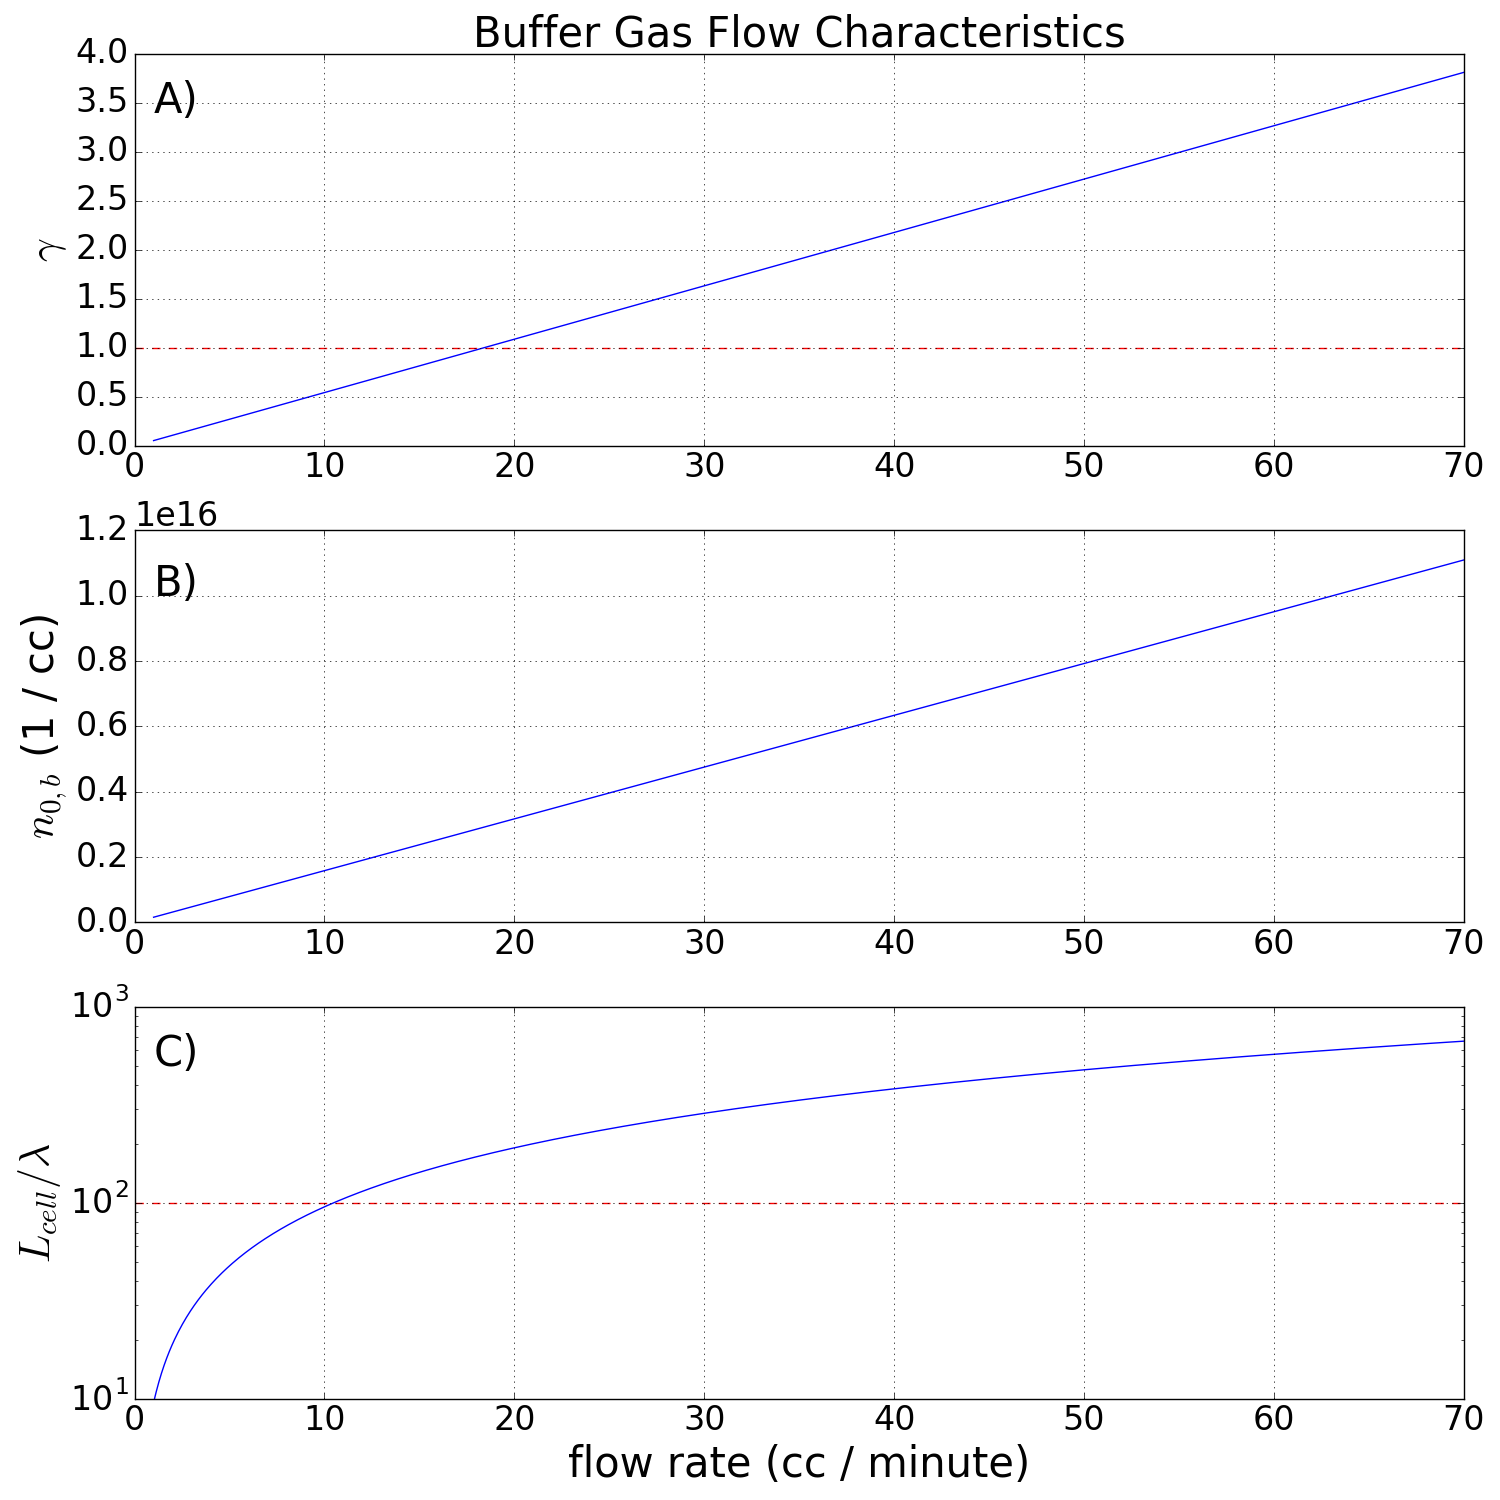
\includegraphics[width=1\textwidth]{Buffer_Gas_Flow_Characteristics.png}
\caption{A) $\gamma$ extraction ratio, dotted red line indicates $\gamma = 1$ where hydrodynamic entrainment begins. B) Theoretical number density of buffer gas species within buffer gas cell. C) Number of collisions one would expect before extraction out of the cell, dotted red line indicates 100 collisions before extraction when rotational degrees of freedom should be thermalized.}
\label{f: buffer_gas_flow}
\end{figure}

\subsection{Beam Density}

With our current capabilities, getting a good read on the beam density is difficult, we do not have a reliable method of characterizing the density at the trap region. We have utilized a residual gas analyzer (RGA) to determine the density of the beam in the ballistic regime upstream from the ion trap. Inserting the RGA into the beam path allows us to estimate the density of water in the beam as a function of the nominal buffer gas flow rate, as shown in figure \ref{f: rga}. Using that fit, we find good agreement with the theoretical calculations showing our flow to be near the supersonic regime, while staying in the hydrodynamic regime with a linear extraction efficiency dependence with the flow rate expressed in \ref{e: gamma}.

\begin{figure}[H]
\centering
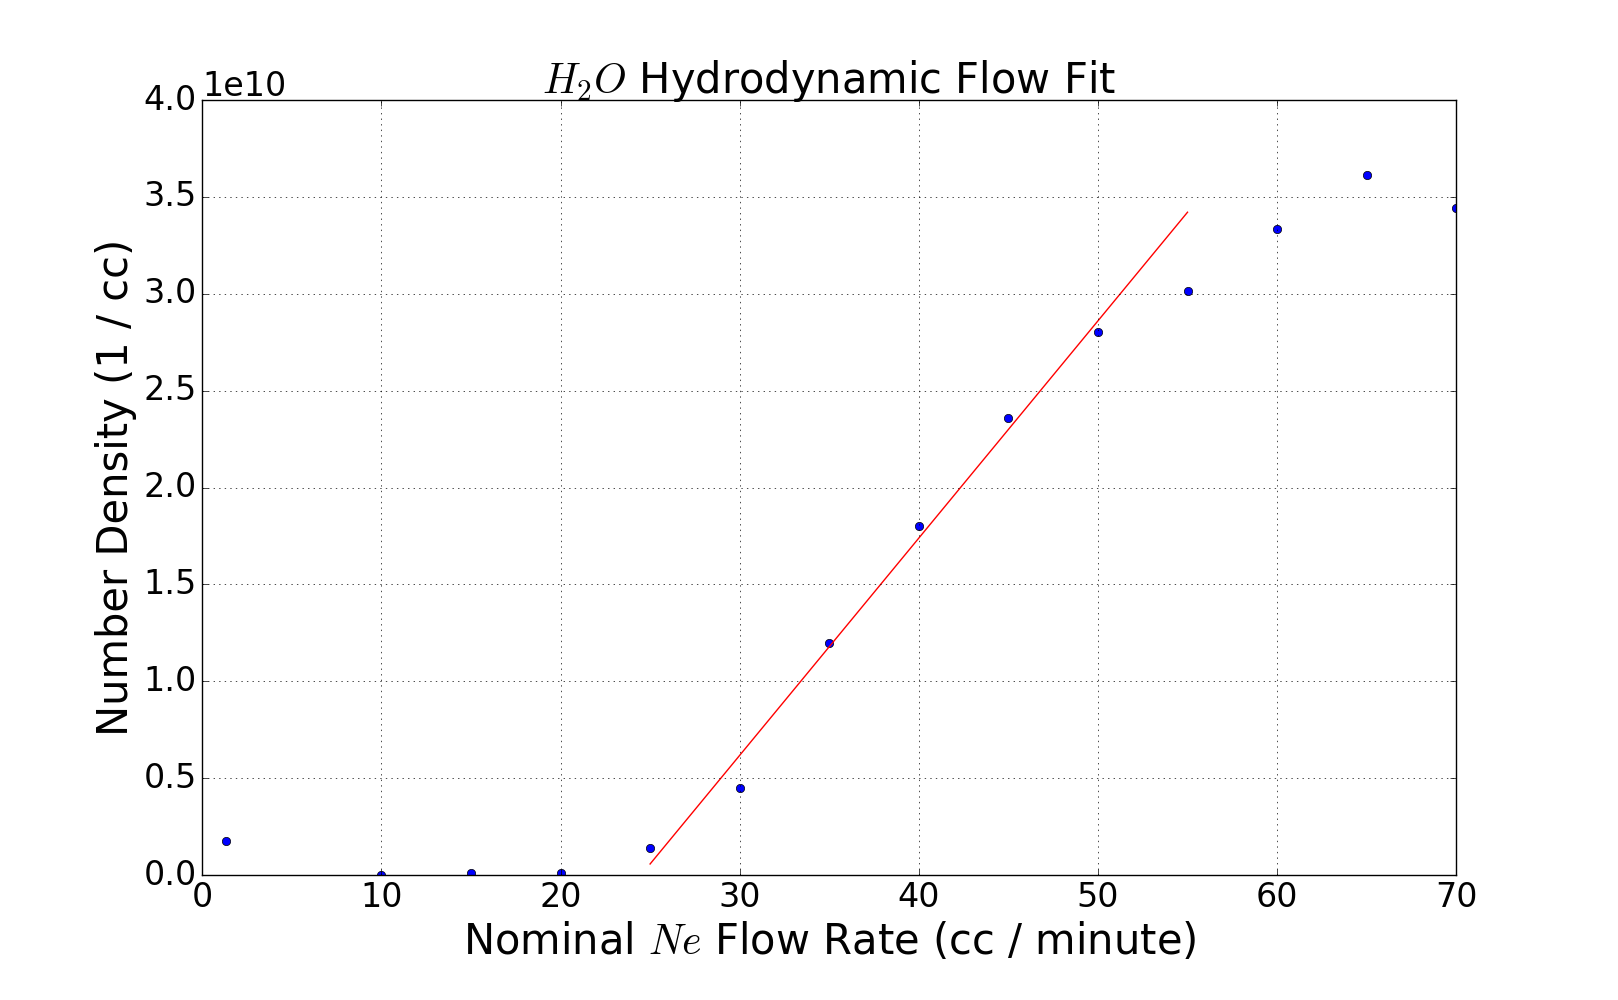
\includegraphics[width=1\textwidth]{hydrodynamic_fit.png}
\caption{}
\label{f: rga}
\end{figure}

\begin{figure}[H]
\centering
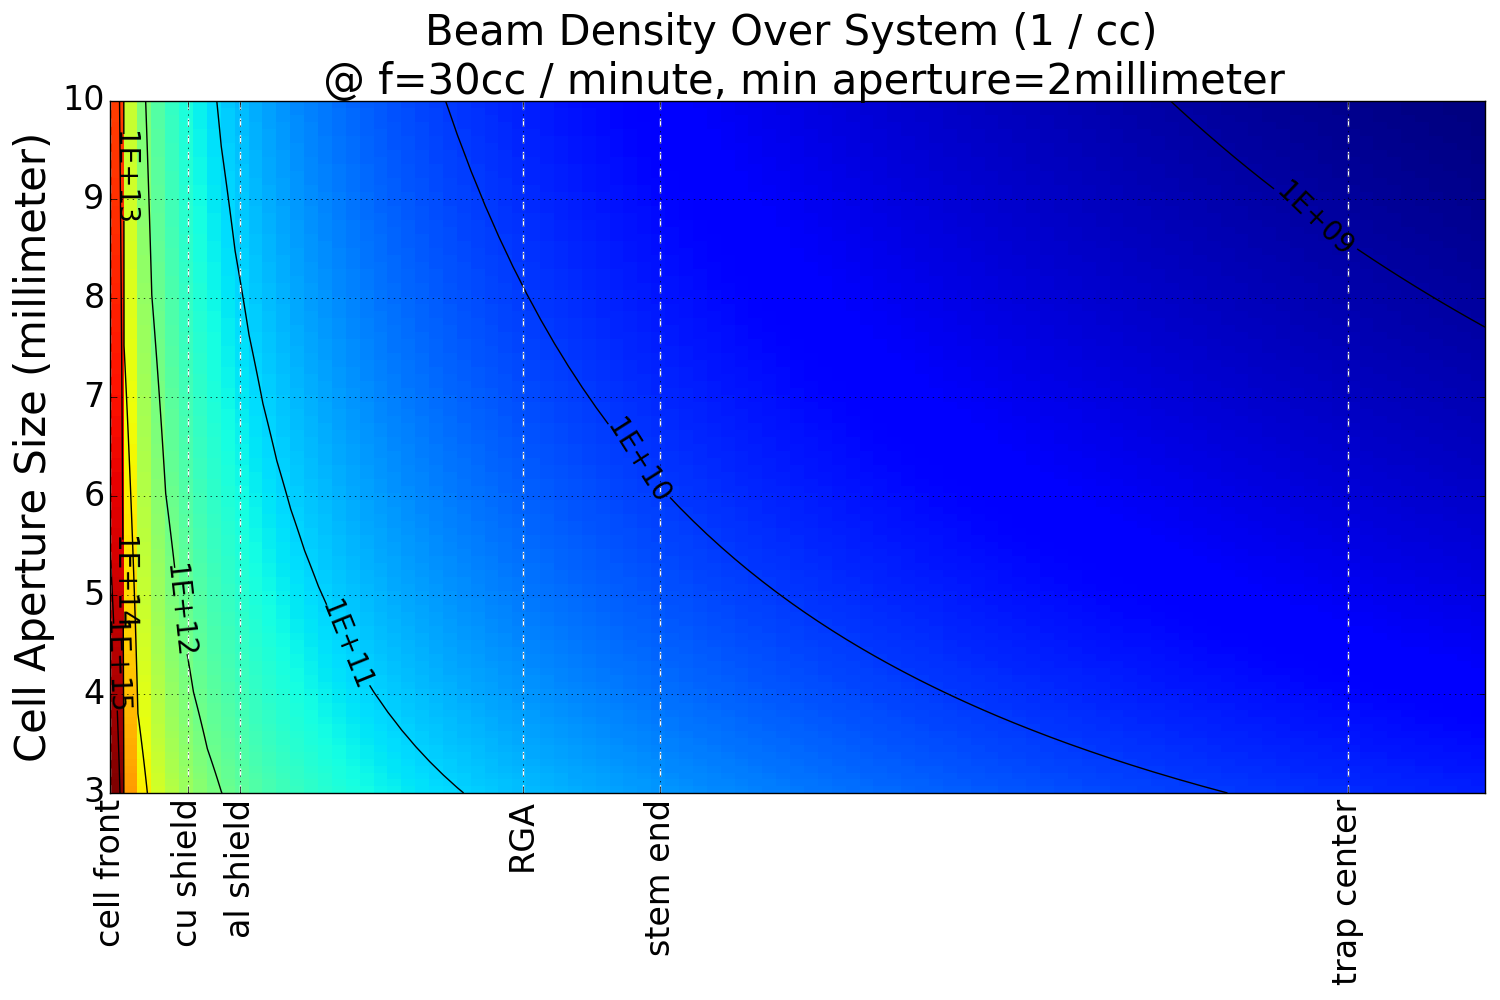
\includegraphics[width=1\textwidth]{beam_density_over_system.png}
\caption{}
\label{f: beam_density}
\end{figure}

Extrapolating the fit and estimated density from figure \ref{f: rga}, we can estimate the density of the water at various locations along the beam line as shown in figure \ref{f: beam_density}. We find that we should be able to produce an appreciable number density of water down at the trap center.

From the RGA, we were able to open and close a shutter in the beam path and see an extinction of the water signal, but a more accurate representation would be from the ions in the trap themselves. We know that the trapped $Be^+$ ions will reaction with $H_2O$ to predominately produce $BeOH$, which we see as a drop in the fluorescence. Figure \ref{f: shutter_closing} shows fits of the fluorescence decay as a beam from the CBGB is suddenly blocked by our shutter in the beam line. Comparing the fitted reaction rates, we find that they agree with the background rates found as shown in figure \ref{f: shutter_bkg}. This indicates to us that we indeed have a beam of cryogenic water coming from the CBGB, as seen by the sudden extinction of the $Be^+ + H_2O$ reaction.

\begin{figure}[H] \label{f: shutter_bkg}
\centering
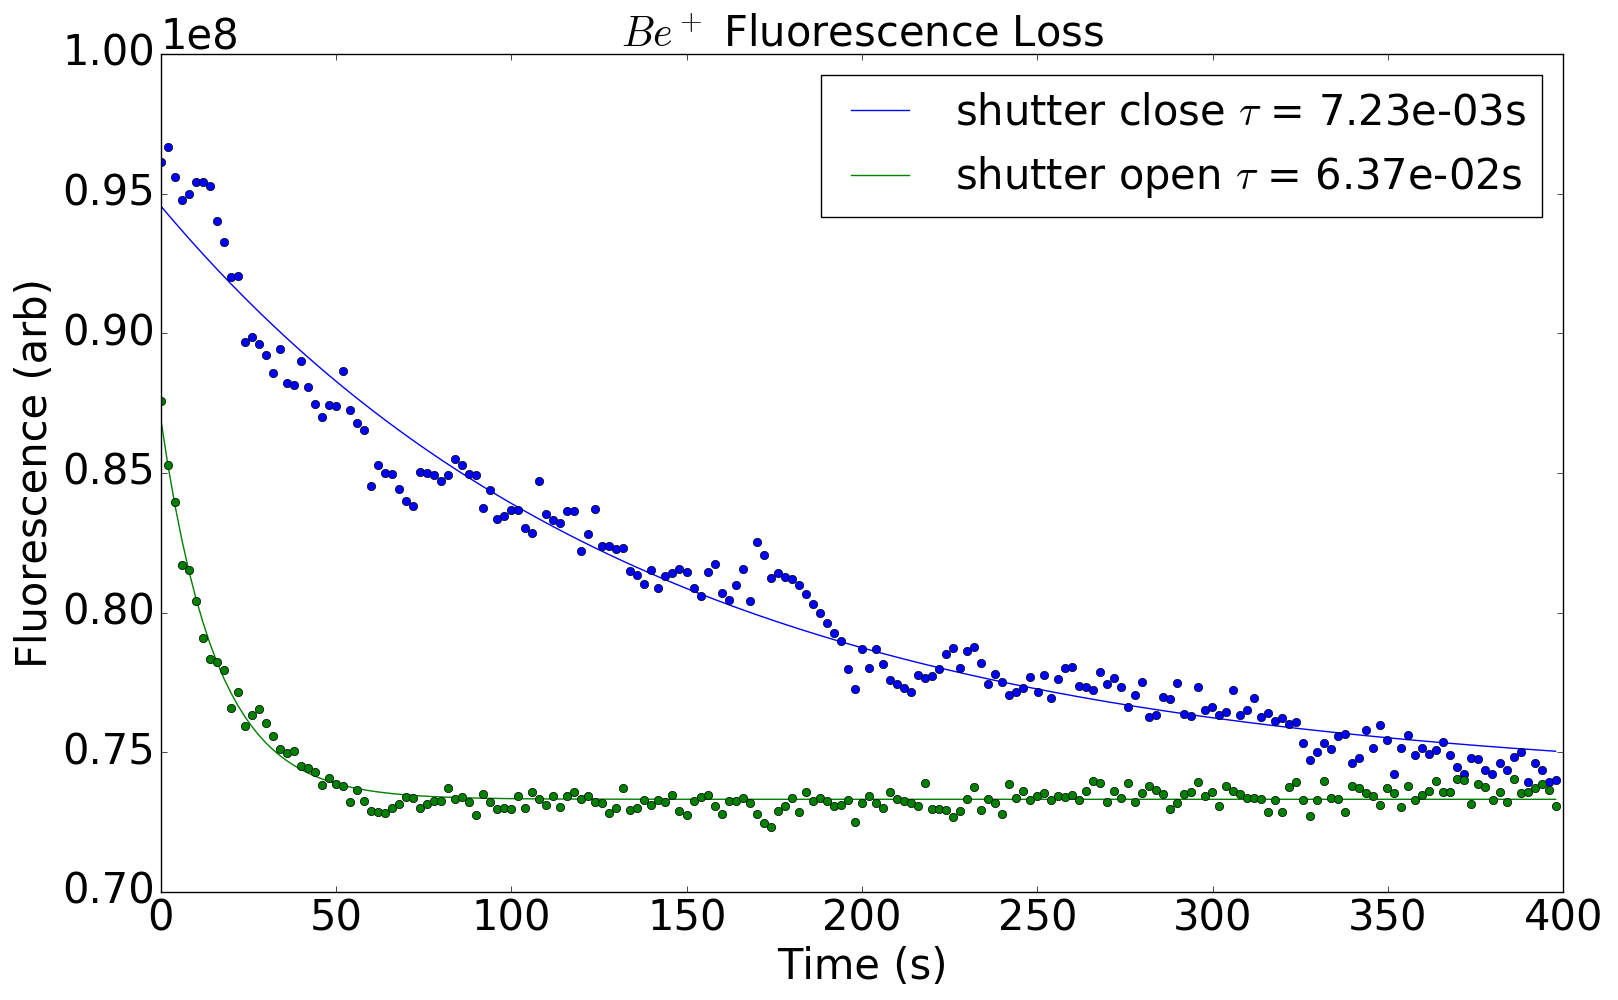
\includegraphics[width=1\textwidth]{sudden_shutter_flow_15_bkg.png}
\caption{}
\end{figure}

\begin{figure}[H] \label{f: shutter_closing}
\centering
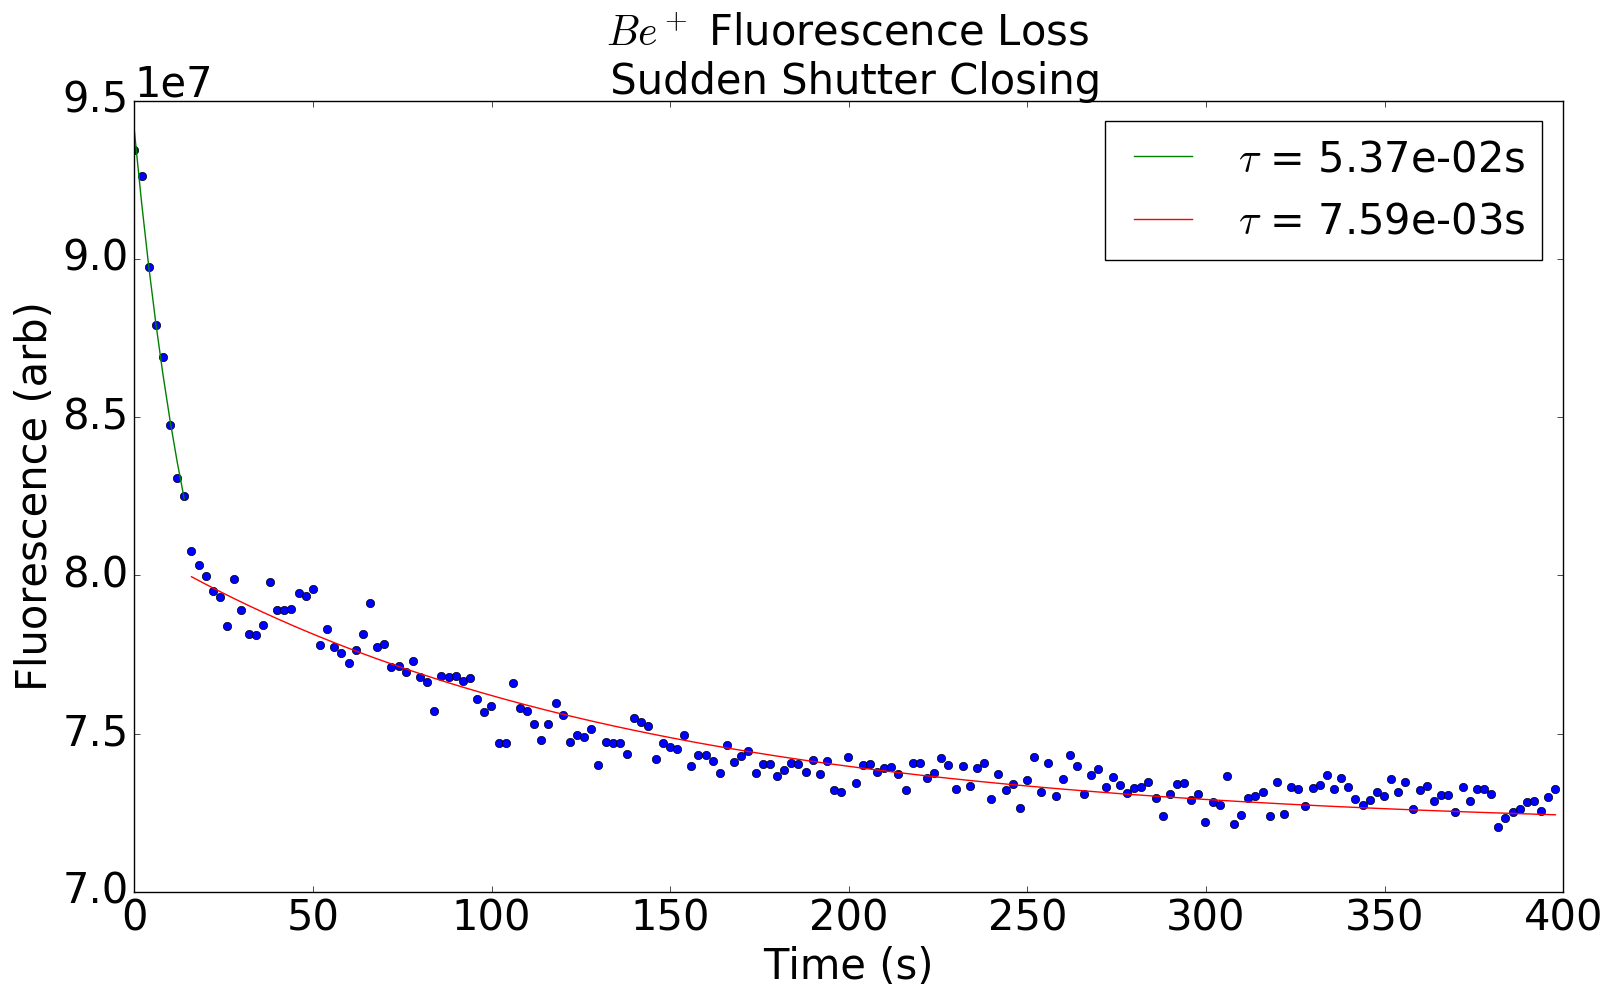
\includegraphics[width=1\textwidth]{sudden_shutter_flow_15_6.png}
\caption{}
\end{figure}

\subsection{Beam velocity}

To better understand the reaction temperatures we will be able to reach, we need a characterization of the beam's velocity, more specifically, the velocity of the target species entrained within the buffer gas. By ablating ytterbium into the neon buffer gas, we find that the ytterbium is entrained within the neon and sympathetically cooled to the cell's temperature. As long as the target species number density is a trace amount in comparison to the bulk buffer gas number density (1:1000), the flow characteristics are dominated by the buffer gas species \cite{Hutzler2012}. The forward velocity of the beam is not only parameterized by the temperature of the buffer gas species, it is also dependent on the flow regime. As we increase the flow of neon into the cell, figure \ref{f: rga} shows a linear increase in the $H_2O$ signal from a downstream RGA. This coincides with the beam operating within the intermediate flow regime, where there are few collisions at the cell aperture, resulting in a slight forward boosting and increased extraction efficiency of the target species. At higher flow regimes, entering the supersonic regime, we would see a "freeze out" where the forward velocity reaches $1.4\bar{v}$ and we would not see appreciable gains in species extraction \cite{Hutzler2012}. We chose to operate at a nominal neon flow rate of 30 sccm based upon the reaction rate of the ions downstream.

\begin{figure}[H]
\centering
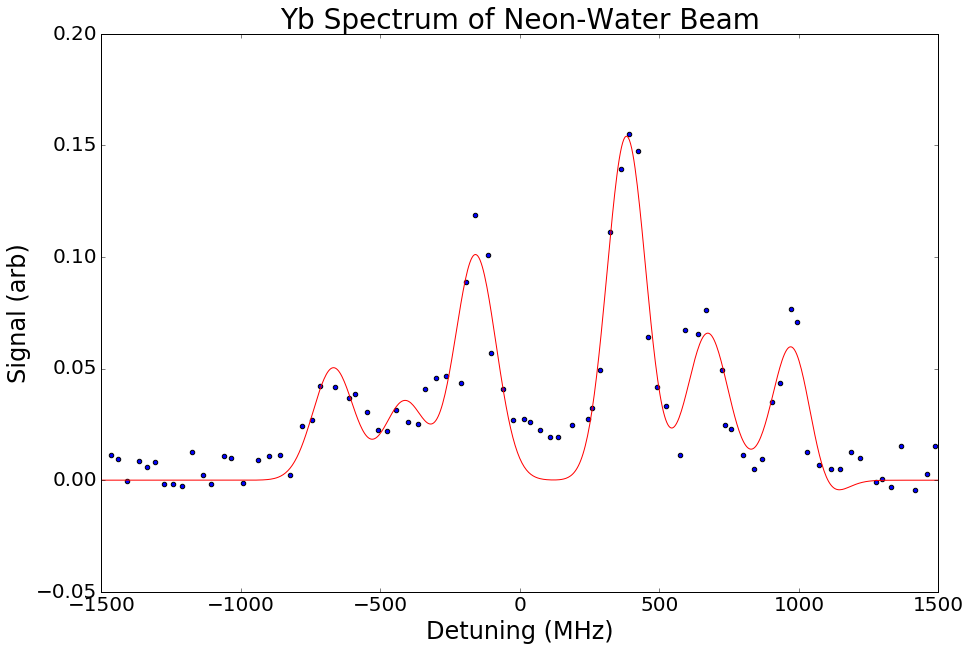
\includegraphics[width=1\textwidth]{yb_spectrum_long.png}
\caption{\label{f: yb_spectrum}}
\end{figure}


\bibliographystyle{abbrv}
\bibliography{Mendeley}

\end{document}